\documentclass[12pt,article]{article}
\usepackage[T1]{fontenc}
\usepackage{lmodern}
\usepackage{longtable}
\usepackage{amssymb,amsmath}
\usepackage{ifxetex,ifluatex}
\usepackage{fixltx2e} % provides \textsubscript
% use upquote if available, for straight quotes in verbatim environments
\IfFileExists{upquote.sty}{\usepackage{upquote}}{}
\ifnum 0\ifxetex 1\fi\ifluatex 1\fi=0 % if pdftex
  \usepackage[utf8]{inputenc}
\else % if luatex or xelatex
  \ifxetex
    \usepackage{mathspec}
    \usepackage{xltxtra,xunicode}
  \else
    \usepackage{fontspec}
  \fi
  \defaultfontfeatures{Mapping=tex-text,Scale=MatchLowercase}
  \newcommand{\euro}{€}
\fi
% use microtype if available
\IfFileExists{microtype.sty}{\usepackage{microtype}}{}
\usepackage[margin=1in]{geometry}
\usepackage{graphicx}
% Redefine \includegraphics so that, unless explicit options are
% given, the image width will not exceed the width of the page.
% Images get their normal width if they fit onto the page, but
% are scaled down if they would overflow the margins.
\makeatletter
\def\ScaleIfNeeded{%
  \ifdim\Gin@nat@width>\linewidth
    \linewidth
  \else
    \Gin@nat@width
  \fi
}
\makeatother
\let\Oldincludegraphics\includegraphics
{%
 \catcode`\@=11\relax%
 \gdef\includegraphics{\@ifnextchar[{\Oldincludegraphics}{\Oldincludegraphics[width=\ScaleIfNeeded]}}%
}%
\ifxetex
  \usepackage[setpagesize=false, % page size defined by xetex
              unicode=false, % unicode breaks when used with xetex
              xetex]{hyperref}
\else
  \usepackage[unicode=true]{hyperref}
\fi
\hypersetup{breaklinks=true,
            bookmarks=true,
            pdfauthor={},
            pdftitle={Are Stand Your Ground Laws Racist and Sexist? A Statistical Analysis of Cases in Florida, 2006-2013},
            colorlinks=true,
            citecolor=blue,
            urlcolor=blue,
            linkcolor=blue,
            pdfborder={0 0 0}}
\urlstyle{same}  % don't use monospace font for urls
\setlength{\parindent}{0pt}
\setlength{\parskip}{6pt plus 2pt minus 1pt}
\setlength{\emergencystretch}{3em}  % prevent overfull lines
\setcounter{secnumdepth}{0}

%%% Change title format to be more compact
\usepackage{titling}
\setlength{\droptitle}{-2em}
  \title{Are ``Stand Your Ground'' Laws Racist and Sexist? A Statistical Analysis
of Cases in Florida, 2006-2013}
  \pretitle{\vspace{\droptitle}\centering\huge}
  \posttitle{\par}
  \author{}
  \preauthor{}\postauthor{}
  \date{}
  \predate{}\postdate{}


\usepackage{dcolumn}
\usepackage{setspace}


\begin{document}

\maketitle


\begin{abstract}
Objective: I test for racial and gender bias in the enforcement of ``stand your ground" (SYG) laws, controlling for potential confounders often invoked to reject claims of racism and sexism. Method: Regressions, simulations, and genetic matching are conducted using case-level data from 237 incidents in the US state of Florida between 2006 and 2013. Results: Controlling for potential confounders, the probability of conviction for a white defendant against a white victim is an estimated 90\% with much error; for a black defendant it is nearly 100\% with little error. For a male defendant in a domestic case, the probability is 40\% whereas for a female defendant it is 80\%. Conclusions: Enforcement of SYG laws appears biased against people of color in general and women specifically in the home. Policy implications are especially stark because these findings contradict recent research conducted for the US Senate.\end{abstract}
\doublespacing

``Stand your ground'' (SYG) laws, which empower individuals to use any
force necessary to defend themselves against anyone they believe to be
an imminent threat, have become one of the most polarizing legal
institutions in the United States. Supporters of SYG laws argue that
they empower self-defense and deter crime (Lott 2013), however, a more
critical view suggests that SYG laws enforce white supremacy over people
of color and male supremacy over female domestic partners, as SYG laws
appear more frequently to benefit white people relative to people of
color (Hundley, Martin, and Humburg 2012; Martin, Hundley, and Humburg
2012) and to only infrequently benefit females (Carmon 2014) or female
survivors of domestic violence in particular (Flatow 2014).

\setlength\parindent{24pt}

This article presents the first systematic statistical analysis of
racial and gender bias in the outcome of SYG cases to control for a wide
variety of contextual factors. The data is gathered from the \emph{Tampa
Bay Times} website, which reports information on 237 cases from the
state of Florida in which an SYG defense was claimed.

Two results from the analysis are notable. First, an SYG defense has
\emph{nearly zero} probability of succeeding when the victim is white
and the defendant is a person of color. This finding remains true after
accounting for more than ten objective factors related to the crime,
suggesting that the racial disparity is not due to any commonly
suspected objective factor correlated with race. Second, when attention
is focused on domestic cases in particular, an SYG defense has a
drastically lower likelihood of succeeding for female defendants
relative to male defendants.

The article proceeds in five sections. The first section provides
background on the controversy surrounding SYG laws and highlights the
main findings of previous research, focusing on previous statistical
analyses. The second section provides a detailed description of the data
and modeling strategy used in this article. The subsequent section
presents the main statistical findings, including two simulation
exercises designed to shed light on two recent, high-visibility cases.
The penultimate section assesses the robustness of the main findings and
a final section concludes.

\subsection{Background and Literature
Review}\label{background-and-literature-review}

``Stand your ground'' laws, adopted by most US states, are laws which
suggest that individuals have no duty to retreat from any place they
have lawful right to be and may use any type of force to defend
themselves, including lethal force, if they reasonably believe they face
an imminent threat of bodily harm. Two recent legal cases dramatize the
criticism of SYG laws. In the trial for the murder of black male
teenager Trayvon Martin, George Zimmerman (an Hispanic male of 28 years)
asked for immunity on SYG grounds. Although this request was not
granted, George Zimmerman was acquitted by a jury and it has been shown
that Florida's SYG laws helped Zimmerman's prospects throughout the
legal process, from the initial police response to the wording of jury
instructions (Coates 2013). On the other hand, Marissa Alexander (a
31-year-old black woman) was convicted of aggravated assault with a
deadly weapon for shooting one warning shot to defend herself against
her husband, despite her claims to self-defense under the same SYG laws
which assisted George Zimmerman toward his acquittal.\footnote{Marissa
  Alexander originally appealed this verdict before ultimately accepting
  a plea deal.}

The \emph{Tampa Bay Times} has organized several key facts regarding all
the cases they could find in which someone from the state of Florida has
claimed an SYG defense since 2006 (``Florida's Stand Your Ground Law''
2013). The \emph{Tampa Bay Times} produced several analyses of their
data, however, their analyses only look at descriptive cross-sections of
the data. They explore the data revealingly, but because they do not
control for other possible explanations their analyses remain vulnerable
to many common, conservative retorts. In particular, it is commonly
argued that bias in outcomes may be due to objective differences which
are merely correlated with race, and that people of color are more
likely to be convicted simply because they are more likely to engage in
violent gun crime (Lott 2013). As the \emph{Tampa Bay Times} must
concede, ``The \emph{Times} analysis does not prove that race caused the
disparity between cases with black and white victims. Other factors may
be at play (Martin, Hundley, and Humburg 2012).''

The only previous statistical test of bias in the enforcement of SYG
laws which sought to control for alternative explanations at the
individual level was an analysis by gun advocate John Lott submitted in
testimony to the US Senate Judiciary Committee (Lott 2013). Using the
data collected by the \emph{Tampa Bay Times}, Lott conducts two logistic
regression analyses on the probability a defendant will be convicted
when SYG is argued. On the basis of these two regression analyses, Lott
submits that there is no evidence of racial bias in SYG cases. However,
Lott's statistical analysis is problematic in several important ways.

The first problem is that the analysis does not provide any discussion
of how the \emph{Tampa Bay Times} data were pre-processed for analysis.
As will become clear in the section below on Data and Method, organizing
the \emph{Tampa Bay Times} data for statistical analysis requires the
analyst to make several non-trivial and non-obvious decisions. However,
the analysis submitted in the US Senate testimony provides no such
discussion. As only one example, the \emph{Tampa Bay Times} provides
several categories for the legal outcome of cases, including
``conviction'' but also ``plea'', ``acquittal'', ``immunity'', etc. The
distinction between what should be counted as ``conviction'' and ``not
conviction'' is far from obvious and, as with all statistical analysis,
requires reasoned argument and transparency from the analyst. Yet, Lott
provides no discussion.Second, his models only include as many as 78 of
the total 237 cases. Because there is no discussion of the data cleaning
process, it is unclear why the analysis is conducted on less than one
third of the total cases, but it leaves open the significant question of
whether one might find different results if more cases were to be
included. Third, both of his two regression models are overfit, with
each one having at least one case completely determined by the
predictors. Regression analysis assumes that the dependent variable is a
function of several predictors and some error term or, in other words,
it assumes a systematic and stochastic component in the process that
generated the dependent variable. Overfitting means that for some cases
there is no error or stochastic component; it is a problem because it
effectively means that some of the predictors in the model are
interpreting error (noise) as a systematic association with predictors
(signal). For this reason, overfit models are known to have poor
predictive performance. Fourth, he does not include several variables
recorded by the \emph{Tampa Bay Times} which are plausible predictors of
outcomes, such as gender and age of victims and defendants, the county
in which the incident occurred, weapon used by defendant, or whether the
victim died.

Most published academic studies of SYG laws have focused on the effect
of SYG laws on homicide rates rather than possible racism in
enforcement. For instance, Cheng and Hoekstra (2013) find that SYG laws
fail to deter burglary, robbery, or assault but increase murder rates by
about 8 percent on net. McClellan and Tekin (2012) also find that SYG
laws lead to an increase of homicides but that the victims are
disproprtionately white males.

The only previous study which focuses on the effect of SYG laws on
racial disparities in legal outcomes is one by Roman (2013), which uses
data from the Federal Bureau of Investigations Supplementary Homicide
Report to model the ruling of justified homicides. Roman reports robust
evidence of racial bias, finding that, compared to white-on-white
homicides, black-on-white homicides have about half the odds of being
ruled justified and that this disparity is worse in states with SYG laws
(Roman 2013, 9). While Roman's findings appear robust, that study has
two key limitations. The first is that the effect of SYG laws is only
considered at the state level as a factor which shapes individual
rulings of justifiable homicide. For this reason the analysis does not
give us direct insight into the subset of cases which specifically
involve SYG claims. The second shortcoming is that Roman is unable to
control for important facts related to the specific cases. This is
crucial because--as many conservative pundits argue and Roman rightly
acknowledges--\emph{if} white-on-black homicides are more likely to be
legitimate cases of self-defense than black-on-white homicides, then
racial disparity in rulings of justifiable homicide may not reflect
racism but rather objective differences in crime rates across racial
groups. Because the \emph{Tampa Bay Times} data contains information on
precisely such contextual factors, the present study allows us to
control for several of the possibly non-racial reasons for this racial
disparity.

\subsection{Data and Methodoloy}\label{data-and-methodoloy}

To test for the possibility of racial and gender bias in SYG cases, I
gathered and processed all the relevant data made available on the
\emph{Tampa Bay Times} website (``Florida's Stand Your Ground Law''
2013).\footnote{I began by downloading a spreadsheet made available on
  the \emph{Tampa Bay Times} website, which included only a small subset
  of the relevant variables included elsewhere on their website. To
  supplement this spreadsheet with the other factors available only
  through the separate webpages for each individual case, I used
  \href{http://import.io}{Import.IO} to crawl and scrape the webpage of
  each case automatically. I then merged, cleaned, and pre-processed the
  spreadsheet made available by the \emph{Times} and the spreadsheet of
  scraped information. All of the raw data and the code necessary to
  reproduce the findings below are available in the replication archive.}
The final result is a data matrix of 175 observations. The data matrix
contains indicators for all the following factors related to each case,
as determined by the questions asked and answered by the \emph{Tampa Bay
Times}, with the names I assigned each variable in parentheses. Did the
victim initiate the incident (Victim Initiated)? Could the defendant
retreat (Defendant Could Retreat)? Did the defendant pursue the victim
(Defendant Pursued)? Did the defendant have a gun (Defendant Gun)? Did
the incident take place on the defendant's property (Defendant's
Property)? Was the victim killed (Deaths)? How old was the victim and
defendant (Victim Age, Defendant Age)? Was there physical evidence
(Physical Evidence)? Was there at least one witness (Witness)? Was the
victim committing a crime (Victim Crime)? Were the victim and defendant
white or non-white (Victim Race, Defendant Race)?\footnote{The decision
  to consider Black and Hispanic people together is imperfect and
  arguable, but seems to me justified by two concerns. First, this seems
  theoretically justified given that the concept of white supremacy
  suggests the primary racial distinction is between white and non-white
  groups. Second, considering that the analysis is already concerned
  with multiple interactions and the sample of data is not exceedingly
  large, considering Black and Hispanic people together simplifies an
  already complex analysis and saves limited degrees of freedom. Future
  research may explore whether disaggregating the race variables leads
  to different results.} Were the victim and defendant female or male
(Victim Male, Defendant Male)?\footnote{Transgender identities were not
  gauged.} Was the incident a domestic dispute (Domestic)? Which county
did the incident occur in (County)? Is there a time trend (Year)?

For the present analysis, conviction refers to any case in which the
defendant received a guilty verdict or took a plea deal; non-convictions
refer to any case in which the defendant was acquitted, dismissed,
granted immunity, or not charged. The inclusion of plea deals with guilty verdicts is not ideal because those who take pleas are not necessarily guilty. I considered removing plea deals row-wise but, given that they are almost as frequent as guilty verdicts (33, and 40, respectively), it does not seem that the improvement of the measure would be so great as to outweigh the loss of information from row-wise deletion. Furthermore, including plea deals with guilty verdicts is theoretically sensible because pleas are likely driven by the expectation that the defendant would be found guilty if tried. Of course, racial identity might shape whether a defendant fears they will be found guilty (innocent or not), but if that is the case then that is precisely why it is best to keep that information in the category of conviction. Ultimately, although plea deals and guilty verdicts are different paths to conviction, they are equally well captured by the concept of conviction insofar as they are both outcomes in which the criminal justice system classifies the defendant as guilty.
  
\pagebreak

\singlespacing

{\footnotesize
\begin{longtable}{lrrrrrrr}
\caption{Summary statistics for numerical variables} \\
 \textbf{Variable} & $\mathbf{n}$ & \textbf{Min} & $\mathbf{\widetilde{x}}$ & $\mathbf{\bar{x}}$ & \textbf{Max} & $\mathbf{s}$ & \textbf{\#NA} \\ 
  \hline
  victim\_age & 175 &   15 &   30 &   32.1 &   79 & 12.8 & 0 \\ 
  accused\_age & 175 &   14 &   35 &   37.1 &   81 & 14.6 & 0 \\ 
  year & 175 & 2005 & 2009 & 2009.1 & 2013 &  2.0 & 0 \\ \hline
\label{Summary statistics for numerical variables}
\end{longtable}
}
{\footnotesize
\begin{longtable}{ll|rrr}
\caption{Summary statistics for categorical variables} \\ 
 \textbf{Variable} & \textbf{Levels} & $\mathbf{n}$ & $\mathbf{\%}$ & $\mathbf{\sum \%}$ \\ 
  \hline
victim\_initiated & Victim did not clearly initiate & 96 & 54.9 & 54.9 \\ 
   & Victim initiated & 79 & 45.1 & 100.0 \\ 
\hline
victim\_crime & Victim was not clearly committing a crime & 137 & 78.3 & 78.3 \\ 
   & Victim was committing a crime & 38 & 21.7 & 100.0 \\ 
\hline
victim\_unarmed & Victim not clearly unarmed & 50 & 28.6 & 28.6 \\ 
   & Victim clearly unarmed & 125 & 71.4 & 100.0 \\ 
\hline
defendant\_pursued & Defendant did not clearly pursue & 126 & 72.0 & 72.0 \\ 
   & Defendant pursued & 49 & 28.0 & 100.0 \\ 
\hline
could\_retreat & Defendant could not clearly have retreated & 72 & 41.1 & 41.1 \\ 
   & Defendant could have retreated & 103 & 58.9 & 100.0 \\ 
\hline
accused\_weapon & Defendant did not clearly have a gun & 63 & 36.0 & 36.0 \\ 
   & Defendant clearly had a gun & 112 & 64.0 & 100.0 \\ 
\hline
deaths & Victim was not killed & 75 & 42.9 & 42.9 \\ 
   & Victim was killed & 100 & 57.1 & 100.0 \\ 
\hline
witness & No clear witness(es)               & 63 & 36.0 & 36.0 \\ 
   & Clear witness(es) & 112 & 64.0 & 100.0 \\ 
\hline
physical\_evidence & No clear physical evidence & 80 & 45.7 & 45.7 \\ 
   & Physical evidence & 95 & 54.3 & 100.0 \\ 
\hline
defendant\_property & Not clearly on property of the defendant & 117 & 66.9 & 66.9 \\ 
   & On property of the defendant & 58 & 33.1 & 100.0 \\ 
\hline
type & Non-domestic                                                                      & 144 & 82.3 & 82.3 \\ 
   & Domestic & 31 & 17.7 & 100.0 \\ 
\hline
victim\_race & Non-white victim & 69 & 39.4 & 39.4 \\ 
   & White victim & 106 & 60.6 & 100.0 \\ 
\hline
victim\_gender & Female victim & 9 & 5.1 & 5.1 \\ 
   & Male victim & 166 & 94.9 & 100.0 \\ 
\hline
accused\_race & Non-white defendant & 65 & 37.1 & 37.1 \\ 
   & White defendant & 110 & 62.9 & 100.0 \\ 
\hline
accused\_gender & Female defendant & 20 & 11.4 & 11.4 \\ 
   & Male defendant & 155 & 88.6 & 100.0 \\ 
   \hline
  \multicolumn{5}{l}{Note: For brevity, the variable \emph{County} is omitted.} \\ \hline
\label{Summary statistics for categorical variables}
\end{longtable}
}
  
\doublespacing

Many variables included different categories to indicate uncertainty,
such as ``disputed'', ``unknown'', or ``unclear.'' In these cases, I
adopted a principle of giving benefit of the doubt to the individual in
question, counting any uncertainty noted by the \emph{Tampa Bay Times}
as not applying to the individual (whether victim or defendant). For
instance, the variable \emph{Witness} is coded such that, if there is
not \emph{clearly} at least one witness confirmed by the \emph{Tampa Bay
Times}, then it takes a value of ``No clear witness(es)'' and otherwise
takes a value of ``Clear witness(es).'' Likewise, the variable
\emph{Victim Crime} takes a value of ``Victim was committing a crime''
in unambiguous cases but a value of ``Victim was not clearly committing
a crime'' whenever the Times noted uncertainty.

After scraping, cleaning, and merging the data from the \emph{Tampa Bay
Times} website, I conducted a series of logistic regression analyses
modeling the odds of conviction as a function of the independent
variables listed above. Logistic regression analysis allows one to
estimate the relationship between multiple independent variables on some
dichotomous outcome.

Following in the spirit of ``intersectional'' perspectives on race and
gender in critical legal research (Crenshaw 1991; Crenshaw 1989), I also
consider the four possible interactions among the race and gender of
defendants and victims (White Victim X White Defendant, Male Victim X
Male Defendant, White Victim X Male Victim, White Defendant X Male
Defendant). I then consider whether domestic cases may have different
effects for male and female defendants (Domestic X Male Defendant), or
for male and female victims (Domestic X Male Victim).

If previously perceived racial or gender bias is simply due to the fact
that one racial group or gender commits more or worse crimes, or because
one racial group or gender more often has to defend itself from certain
types of crimes, then the coefficients related to race or gender should
be statistically indistinguishable from zero while objective factors
related to the incident should be statistically significant predictors
of conviction (e.g., if the victim initiated the incident and was armed,
this should be associated with a lower likelihood of conviction).

\subsection{Analysis}\label{analysis}

Table 1 presents the results from three logistic regression analyses.
Model 1 is a baseline model with all independent variables of interest
included separately, whereas Models 2 and 3 introduce interaction terms
to test whether race and gender condition the independent effects of
certain primary variables. Each coefficient reflects the average change
in log-odds of conviction associated with each corresponding independent
variable. Specifically, each coefficient reflects the expected change in
log-odds of conviction associated with the independent variable taking
the value indicated by the variable's name, relative to the absence or
opposite of that value. Standard errors in parentheses reflect the
statistical uncertainty of the coefficients. Starred coefficients are
those which are very unlikely to be observed merely by chance, according
to conventional cutoffs. For instance, the coefficient for \emph{Victim
Initiated} in Model 1 suggests that, on average, a situation which the
victim initiates has a log-odds of conviction 3.2 less than if the
victim did not clearly initiate, assuming all the other independent
variables are equal to their modal values. Because log-odds are not
conveniently interpretable in terms of substantive effects, I postpone
discussion of effect sizes for the following subsection.

\begin{center}[Insert Table 1 about here.]\end{center}

First, a series of objective factors related to the incident appear to
have clear and intuitively sensible effects on the likelihood of
conviction. Victim initiation appears to have a relatively large and
highly significant negative effect on the likelihood of conviction,
robust across all three models. On the other hand, also intuitively
sensisble, a clear ability for the defendant to retreat is associated
with a significantly greater likelihood of conviction in all three
models. Similarly, death of the victim appears, as we might expect, to
significantly and robustly increase the probability of conviction.
Perhaps surprisingly, however, defendants armed with a gun are
significantly less likely to meet conviction. This is especially
interesting given that conservative critics sometimes suggest that
racial disparities in outcomes are spurious evidence of racism because
people of color may be more likely to use guns in violent crimes (Lott
2013), the assumption being that guns rather than colored skin tend
toward convictions. Although it is purely speculative, one might
hypothesize that the negative association between guns and conviction is
due to the fact that other types of weapons (and unarmed assaults)
require the defendant to engage in overtly active behavior toward the
victim, whereas those armed with guns can assault a victim without
obviously, actively moving toward the victim.

Several independent variables appear to have no relationship with the
likelihood of conviction. It is interesting that, given SYG laws are
often associated with the defense of homes, incidents taking place on
the defendant's property do not appear any less likely to end in
conviction. Witnesses and physical evidence also have no clear effect on
the probability of conviction.

What do the models say about the key variables of interest, race and
gender? In the baseline Model 1, white defendants appear to face a
significantly lower likelihood of conviction (compared to black
defendants) and white victims appear to increase the likelihood of
conviction (compared to black victims), even after controlling for all
of the objective factors considered already. However, if one considers
how the race of both defendants and victims interact (Model 2), the race
of the defendant per se does not appear to have any independent effect
on the probability of conviction. However, crucially, Model 2 suggests
that the extra likelihood of conviction in cases of white victims is
significantly greater for defendants of color compared to white
defendants.\footnote{The statistically significant coefficient of 9.90
  for \emph{Victim White} reflects the expected change in log odds of
  conviction for when the victim is white compared to when the victim is
  a person of color, \emph{while} the defendant is a person of color.
  The negative and significant coefficient for \emph{White Victim X
  White Defendant} suggests that the coefficient of 9.9 associated with
  a white victim decreases by an average of 4.2 for white defendants.
  See below for more conveniently interpretable effect sizes.} Model 2
also suggests that the extra likelihood of conviction in cases of white
victims is significantly greater for female relative to male
victims.\footnote{The negative and significant coefficient for
  \emph{White Victim X Male Victim} suggests that the coefficient of 9.9
  associated with a white victim decreases by an average of 6.0 for male
  victims relative to female victims.}

The coefficients for \emph{Domestic} in Models 1 and 2 suggest that in
general, domestic disputes which involve SYG claims are less likely to
result in conviction. But to test the claim that SYG laws are biased
against women in cases of domestic violence (Flatow 2014), Model 3
introduces the interaction terms \emph{Domestic X Male Defendant} and
\emph{Domestic X Male Victim} to identify whether the domesticity of an
incident depends on the gender of the victim or defendant. The
statistically significant and negative coefficient for \emph{Domestic X
Male Defendant} suggests that the tendency of defendants to escape
conviction in domestic cases is significantly greater for male
defendants compared to female defendants. Furthermore, as evidenced by
the coefficient for \emph{Domestic} in Model 3, the effect of
domesticity on conviction is statistically indistinguishable from zero
when the defendant is female. The gender of the victim, however, has no
discernable conditioning effect on the relationship between domesticity
and conviction.

Before assessing the size of these estimated effects, it should be noted
that in addition to the interaction of race across defendant and victim,
and the interaction of domesticity and gender, it has been argued that
race and gender interact in complicated ways specifically within cases
of domestic violence. Crenshaw highlights in particular that women of
color relative to white women may be less likely to challenge domestic
abuse through the legal system because the home may be seen as a ``safe
haven'' with respect to racism in society, and/or to avoid negative
stereotypes about black communities (Crenshaw 1991, 1257; Crenshaw 1989,
71). Unfortunately, separate analyses attempting to explore this
additional layer of complexity were found to be uninformative due to the
limited size of the present sample.\footnote{Specifically, following in
  the spirit of Crenshaw's arguments, I considered four variations of
  Model 3, focusing on the domesticity-gender interaction for cases of
  white victims only and for cases of non-white victims only. With only
  68 cases of non-white victims, full models similar to those reported
  in Table 1 lead to overfitting. Removing some independent variables
  could avoid overfitting but is typically a bad strategy because it
  increases the risk of omitted variable bias and introduces
  arbitrariness. In the absence of expert, \emph{a priori} knowledge
  regarding the true data generating process, I judged it not worthwhile
  to examine these additional layers of complexity given the present
  data.} However, future research using additional or different data, or
alternative modeling strategies may very well generate valuable insights
which further refine the general findings presented here.

\pagebreak

\begin{center}[Insert Figure 1 about here.]\end{center}

Figure 1 illustrates the key estimate of interest from Model 2 in terms
of probability. As the graph reveals, the probability of conviction is
rather high in general when all the variables in Model 2 are assumed to
be at their modal values, but the probability of conviction for
non-white defendants against white victims \emph{approaches 1} and shows
a strikingly smaller margin of error at a 95\% confidence level. In
other words, white defendants against white victims have, on average,
about a 90\% chance of conviction, but nonetheless there is a
significant class of such defendants who are more likely to escape
conviction; whereas, for non-white defendants in otherwise equivalent
cases, there are no cases which are more likely to escape conviction. As
Model 2 reveals, this difference is substantial enough that there is
less than a 5\% probability we would observe this difference due to
random chance alone.

\begin{center}[Insert Figure 2 about here.]\end{center}

Figure 2 illustrates the key estimate of interest from Model 3 in terms
of probability. As the graph indicates, male defendants in domestic
cases are significantly less likely to be convicted than female
defendants in otherwise equivalent domestic cases. With respect to
domestic cases, the gender bias is even more pronounced than the racial
bias indicated in Figure 2. In otherwise comparable cases, the
probability of conviction for male defendants is less than 40\% whereas
the probability of conviction for female defendants is greater than
80\%.

How do these statistical findings speak to the justice of past and
future legal cases? With caution, the analyses presented here can be
used to consider how legal outcomes would be expected to change, on
average, given different racial and gender identities for defendants and
victims. To make the findings more substantively interpretable in light
of publicly well-known cases, I consider two counterfactual questions.
First, how would George Zimmerman's probability of conviction change had
Trayvon Martin been white but all the other objective factors of
the case had been the same as they were? Second, with respect to Marissa
Alexendar's currently on-going appeal against her previous conviction,
how would her probability of conviction change had she been a male
defendant in an otherwise equivalent case?

To consider the case of George Zimmerman, I conducted 1000 simulations
of Model 2 to estimate the probability distribution of conviction in a
2012 case where the defendant is non-white, the defendant is 28 years
old, the victim is non-white, the victim is 17 years old, the victim
died, the defendant clearly had a gun, the victim was clearly unarmed,
the victim was not clearly committing a crime, the defendant actively
pursued the victim, the defendant could have retreated, the defendant
was not clearly on their own property, the victim did not clearly
initiate, there were no clear witnesses, the defendant and victim were
both male, and they were engaged in a non-domestic incident. Based on
the results of the simulation, it is estimated that George Zimmerman's
\emph{ex ante} probability of conviction was 0.69 (sd = 0.21). In other
words, according to Model 2, \emph{ex ante} George Zimmerman was more
likely to be convicted than not, but with a notable margin of error
which made his odds not clearly very much better than those of a coin
flip. In a hypothetical case in which all of these factors are exactly
the same except the victim is white, the expected probability of
conviction is 0.98 (sd = 0.05). In summary, had Trayvon Martin been
white, George Zimmerman's \emph{ex ante} probability of conviction would
have changed by an average of 0.29 (sd=0.19).

To consider the case of Marissa Alexander, I conducted 1000 simulations
of Model 3 to estimate the probability distribution of a defendant being
convicted in a 2010 case where the defendant is non-white, the defendant
is 31 years old, the victim is non-white, the victim is 34 years old,
the victim did not die, the defendant clearly had a gun, the victim was
clearly unarmed, the victim was not clearly committing a crime, the
defendant did not clearly pursue the victim, the defendant could have
retreated, the defendant was not clearly on their own property, the
victim did not clearly initiate, there was at least one clear witness,
and a female defendant and male victim were engaged in a domestic
incident. Based on the results of this exercise, the \emph{ex ante}
expected probability of conviction for Marissa Alexander given the
objective facts of her case was an estimated 0.55 (sd = 0.28). In other
words, according to Model 3, \emph{ex ante} Michelle Alexander was
marginally more likely to be convicted than not but with a margin of
error which made her odds statistically indistinguishable from those of
a coin flip. In a hypothetical case in which all of these factors are
exactly the same except the defendant is male, the expected probability
of conviction becomes 0.14 (sd = 0.14). In summary, had Marissa
Alexander been male, her \emph{ex ante} probability of conviction would
have changed by an average of -0.42 (sd=0.27).

\subsection{Robustness}\label{robustness}

One common problem in regression analysis is that it is possible for
unrepresentative cases to disproportionately drive model results. As the
partial residuals in the effect plots above reveal some noticeable
outliers, I calculate Bonferonni-adjusted p-values for the largest
Studentized residuals in each model using normal distribution tests. In
both models, the largest Studentized residual is not statistically
significant, suggesting that the estimates above are unlikely to be
artifacts of a few odd cases.\footnote{For the sake of brevity numerical
  results are not reported but are reproducible from the replication
  archive.}

A more complicated problem for drawing statistical inferences from
observational data is the possibility that the units of analysis are
distributed into the different values of an independent variable by
other covariates. If some covariate systematically shapes the
probability a unit will take a certain value on the independent variable
of interest, estimates for that independent variable will be biased. To
guard against this problem, I use a genetic matching search algorithm to
automatically create a subset of the original sample which is optimally
balanced on the other covariates (Diamond and Sekhon 2012; Sekhon 2011).
The algorithm identifies the weights which need to be applied to each
covariate (including scores for the propensity to be ``treated'') to
limit the sample to those matched pairs of treatment and control units
which optimize balance on the covariates. From these subsets of cases
the estimated average treatment effect will approximate that which would
be inferred from a randomized experiment, assuming of course that all
relevant covariates have been included in the matching procedures.

Given that the main hypotheses relate to interaction terms, I conduct
the matching procedures only on relevant subsets of the initial sample.
For Model 2, the relevant subset includes only cases with white victims
and the ``treatment'' effect to be estimated is the defendant being a
person of color. For Model 3, the relevant subset includes only domestic
cases and the ``treatment'' effect to be estimated is the defendant
being female.

Before proceeding, note that a drawback of matching techniques is the
significant loss of information that occurrs in the reduction of an
initial sample to only matched pairs. In the present case, this sample
attrition is especially severe for two reasons. First, the original
sample of 175 cases is already small relative to the large number of
covariates including interaction terms. Second, limiting the matching
analysis to subsets in order to straightforwardly estimate treatment
effects for interactive hypotheses reduces the original sample to 106
cases of white victims and 31 domestic cases. For Model 2, the matching
procedures reduce the subset of white-victim cases to a subset of 18
matched observations and for Model 3 the subset of domestic cases is
reduced to 8 matched observations.

Despite the drastic loss of information, matching estimates for both
models are sized consistently with the estimates in the main regression
models and statistically significant. For Model 2, the average treatment
effect from being a defendant of color (in cases with white victims) is
0.26 (standard error = 0.12, p = 0.03). Note that this is a different
effect than that which was estimated in the thought experiment related
to the Trayvon Martin case. There it was asked what the expected effect
would have been had Trayvon Martin been white (varying the race of the
victim), whereas the matching estimates relate to the effect of being a
defendant of color in a case with a white victim (varying the race of
the defendant). Nonetheless the matching estimate of 0.26 appears
consistent with the estimate from Model 2 (about .1) given that the
difference between white defendants and defendants of color in Model 2
was compressed by the relatively high rate of conviction for all
defendants in cases with white victims. Thus considering only matched
pairs in only cases with white victims corroborates the results of Model
2, suggesting that, if anything, the estimated racial effect from Model
2 was biased downward.

For Model 3, the average treatment effect from being a female defendant
(in domestic cases) is 0.62 (standard error = 0.21, p = 0.003). Here the
matching estimate can be directly compared to the thought experiment
relating to the case of Marissa Alexander. The estimated effect after
matching is similar to that derived from Model 3 reported above, from
which it was estimated that had Marissa Alexander been male her
probability of conviction would have changed by -0.42 (sd=0.27). Again
the matching estimate suggests that, if anything, the estimated gender
effect from Model 3 is conservative.

Thus, it is unlikely the estimates presented here are merely artifacts
of outliers or of imbalance in the propensity to be in one of the
relevant treatment groups. The consistency of the effect sizes and their
statistical significance in all cases increases confidence in both of
the key findings.

\subsection{Conclusion}\label{conclusion}

Though many critics argue that ``stand your ground'' (SYG) laws are
characterized by racism and sexism in their outcomes, almost all
research on this question has been unable to control for a wide variety
of other factors which defenders of SYG laws commonly invoke to explain
away the implication of racial or gender bias. The critique of SYG laws
has remained vulnerable to the conservative defense that SYG laws are
not, but only seem to be, racist or sexist because certain racial or
gender types are more or less likely to be involved in certain types of
cases which are objectively more or less likely to end in legitimate
convictions. Indeed, the only previous statistical analysis which sought
to control for a wide variety of objective factors concluded precisely
that there is no racial bias in the outcome of SYG cases after
controlling for other objective factors relevant to each case (Lott
2013).

This research note provides the first properly documented and
systematic, article-length statistical analysis of racial and gender
bias in SYG cases which controls for a wide variety of objective factors
possibly correlated with race and/or gender. In stark contrast to John
Lott's analysis submitted in testimony to the US Senate Judiciary
Committee, I find evidence of both racial and gender bias in a sample of
Florida SYG cases from 2006-2013 reported by the \emph{Tampa Bay Times}
(``Florida's Stand Your Ground Law'' 2013).

In particular, the probability of conviction for a white defendant
against a white victim in a typical case was found to be high at 90\%
(though with a relatively large margin of error) but the probability of
conviction for a black defendant in an otherwise objectively equivalent
case was found to approach 100\% (with a relatively small margin of
error). The gender bias in domestic cases appears to be even more
pronounced. Conviction for a male defendant in a typical domestic case
was found to be about 40\%, but for a female defendant in an otherwise
objectively equivalent case, the probability of conviction was found to
be around 80\%.

To put the findings in perspective, I also used simulations to consider
how the probability of conviction would change in response to changes in
racial and gender identities in two well-known and recent cases. In the
case of George Zimmerman's killing of unarmed black teenager Trayvon
Martin in 2012, I found that if Trayvon Martin had been white the
probability of a conviction would have increased by an estimated 0.29,
from 0.69 to 0.98. With respect to the case of Marissa Alexander's
warning shot against husband Rico Gray in a 2010 domestic dispute, I
found that if Alexander had been a male the probability of a conviction
would have decreased by an estimated 0.42, from 0.55 to 0.14. This
statistical exercise is especially concerning for Michelle Alexander's
case because it reveals that she is not only more likely to be convicted
than a man would, but that \emph{ex ante} her most likely outcome is
qualitatively different than a man's would be in an equivalent case:
Alexander was altogether more likely to be convicted than not, whereas a
man in an objectively equivalent case would not simply be less likely to
be convicted but would also be altogether more likely to go free than be
convicted. Thus, the statistical analysis presented here indicates an
alarmingly high probability that Marissa Alexander's initial conviction
(currently under appeal) was an artifact of institutionalized sexism
(i.e.~patriarchy).

In summary, the analysis presented here provides striking evidence of
both racial and gender bias in the outcomes of Florida cases between
2006-2013 in which ``stand your ground'' laws are invoked. It reveals
fundamental flaws in a previous analysis submitted in testimony to the
US Senate Judiciary Committee (Lott 2013) and finds unreliable its
conclusions of no racial bias. Finally, this research note informs
important public debate about the possibility of racism and sexism in
the application of SYG laws, suggesting that lawmakers and judges have
paid inadequate heed to the racial and gender implications of ``stand
your ground'' laws.

\pagebreak

\begin{table}[!htbp] \centering 
  \caption{Logistic Regressions for Dependent Variable $Conviction$} 
  \label{} 
\scriptsize 
\begin{tabular}{@{\extracolsep{0pt}}lD{.}{.}{-2} D{.}{.}{-2} D{.}{.}{-2} } 
\\[-1.8ex]\hline \\[-1.8ex] 
\\[-1.8ex] & \multicolumn{1}{c}{\textbf{Model 1}} & \multicolumn{1}{c}{\textbf{Model 2}} & \multicolumn{1}{c}{\textbf{Model 3}}\\ 
\hline \\[-1.8ex] 
 Victim Initiated & -3.20^{***} & -3.30^{***} & -3.60^{***} \\ 
  & (0.79) & (0.85) & (0.86) \\ 
  Victim Crime & -0.44 & -1.20 & -0.14 \\ 
  & (0.98) & (1.10) & (1.00) \\ 
  Victim Unarmed & 0.83 & 1.50^{*} & 0.70 \\ 
  & (0.64) & (0.77) & (0.66) \\ 
  Defendant Pursued & -0.29 & -0.33 & -0.50 \\ 
  & (0.67) & (0.72) & (0.71) \\ 
  Defendant Could Retreat & 1.70^{**} & 2.00^{***} & 1.90^{***} \\ 
  & (0.69) & (0.74) & (0.73) \\ 
  Defendant Gun & -1.80^{***} & -1.90^{***} & -2.10^{***} \\ 
  & (0.68) & (0.74) & (0.75) \\ 
  Deaths & 2.60^{***} & 2.70^{***} & 2.90^{***} \\ 
  & (0.71) & (0.79) & (0.77) \\ 
  Witness & -0.32 & -0.12 & -0.20 \\ 
  & (0.63) & (0.71) & (0.67) \\ 
  Physical Evidence & -0.95 & -0.96 & -0.96 \\ 
  & (0.60) & (0.63) & (0.61) \\ 
  Defendant's Property & -0.13 & 0.36 & -0.25 \\ 
  & (0.71) & (0.81) & (0.74) \\ 
  Domestic & -1.70^{*} & -2.40^{**} & 3.90 \\ 
  & (0.88) & (1.00) & (3.00) \\ 
  Victim White & 2.10^{***} & 9.90^{**} & 1.80^{**} \\ 
  & (0.77) & (3.90) & (0.78) \\ 
  Victim Male & -1.40 & 4.50 & -1.40 \\ 
  & (1.30) & (3.80) & (2.00) \\ 
  Victim Age & 0.02 & 0.04 & 0.02 \\ 
  & (0.02) & (0.03) & (0.02) \\ 
  Defendant White & -1.90^{**} & -0.13 & -1.90^{**} \\ 
  & (0.78) & (1.90) & (0.81) \\ 
  Defendant Male & 0.17 & 5.50 & 1.60 \\ 
  & (0.94) & (4.10) & (1.40) \\ 
  Defendant Age & 0.001 & -0.01 & 0.002 \\ 
  & (0.02) & (0.02) & (0.02) \\ 
  White Victim X White Defendant &  & -4.20^{**} &  \\ 
  &  & (1.80) &  \\ 
  Male Victim X Male Defendant &  & -6.10 &  \\ 
  &  & (4.00) &  \\ 
  White Victim X Male Victim &  & -6.00^{*} &  \\ 
  &  & (3.50) &  \\ 
  White Defendant X Male Defendant &  & 0.53 &  \\ 
  &  & (1.80) &  \\ 
  Domestic X Male Defendant &  &  & -4.30^{**} \\ 
  &  &  & (2.10) \\ 
  Domestic X Male Victim &  &  & -2.60 \\ 
  &  &  & (2.90) \\ 
 N & \multicolumn{1}{c}{175} & \multicolumn{1}{c}{175} & \multicolumn{1}{c}{175} \\ 
Log Likelihood & \multicolumn{1}{c}{-58.00} & \multicolumn{1}{c}{-52.00} & \multicolumn{1}{c}{-55.00} \\ 
AIC & \multicolumn{1}{c}{208.00} & \multicolumn{1}{c}{204.00} & \multicolumn{1}{c}{206.00} \\ 
\hline \\[-1.8ex] 
\multicolumn{4}{l}{$^{***}$p $<$ .01; $^{**}$p $<$ .05; $^{*}$p $<$ .1} \\ 
\multicolumn{4}{l}{County and Year variables included in the models but not displayed. Robust (Huber-White) standard errors in parentheses.} \\ 
\end{tabular} 
\end{table}

\pagebreak

\begin{figure}[htbp]
\centering
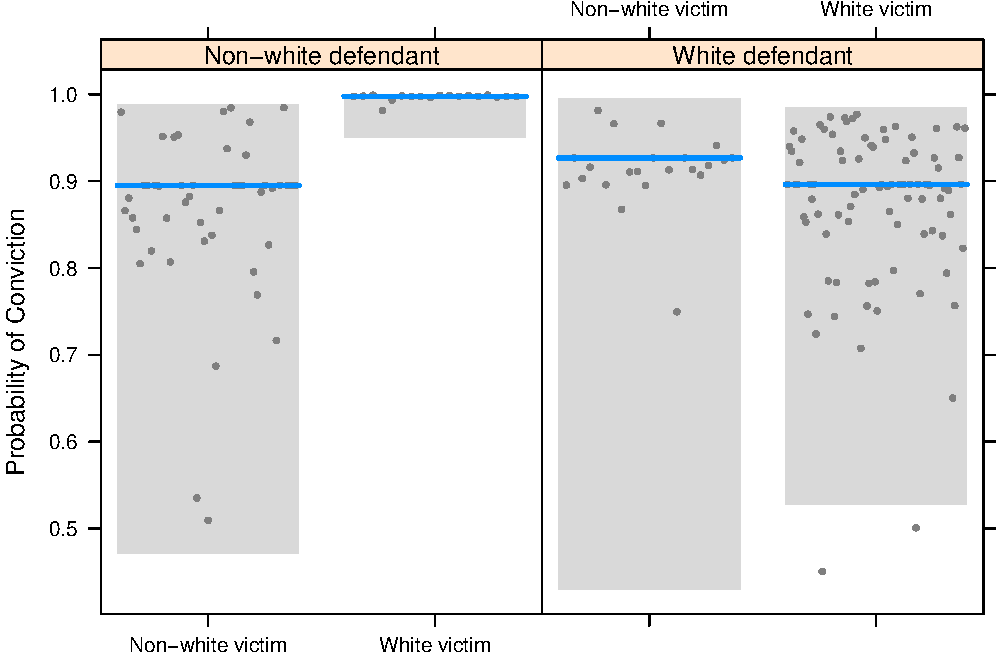
\includegraphics{stand_your_ground_article_files/figure-latex/unnamed-chunk-7.pdf}
\caption{Effect of Victim's Race on Probability of Conviction for White
and Non-White Defendants (95\% Confidence Intervals and Partial
Residuals in Grey)}
\end{figure}

\pagebreak

\begin{figure}[htbp]
\centering
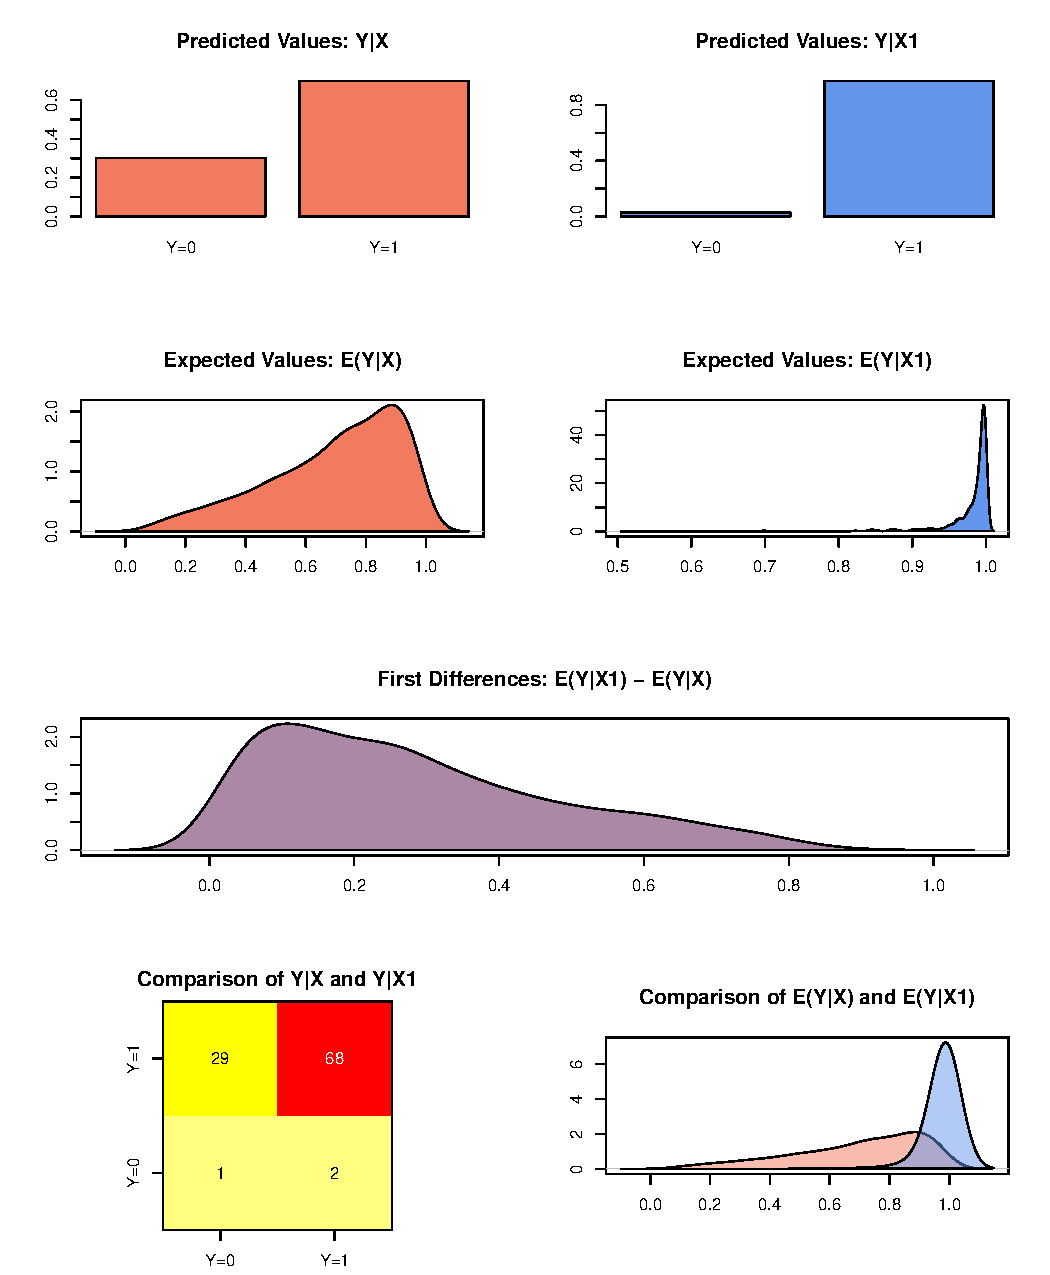
\includegraphics{stand_your_ground_article_files/figure-latex/unnamed-chunk-8.pdf}
\caption{Effect of Domesticity on Probability of Conviction for Male and
Female Defendants (95\% Confidence Intervals and Partial Residuals in
Grey)}
\end{figure}

\pagebreak

\setlength\parindent{0pt}

\subsection*{References}\label{references}
\addcontentsline{toc}{subsection}{References}

Carmon, Irin. 2014. ``Can Women Stand Their Ground? Depends on the
Target.'' \emph{MSNBC}, March.
\url{http://www.msnbc.com/msnbc/can-women-stand-their-ground}.

Cheng, Cheng, and Mark Hoekstra. 2013. ``Does Strengthening Self-Defense
Law Deter Crime or Escalate Violence? Evidence from Expansions to Castle
Doctrine.'' \emph{Journal of Human Resources} 48 (3): 821--54.

Coates, Ta-Nehisi. 2013. ``How Stand Your Ground Relates To George
Zimmerman.'' \emph{The Atlantic}, July.
\url{http://www.theatlantic.com/national/archive/2013/07/how-stand-your-ground-relates-to-george-zimmerman/277829/}.

Crenshaw, Kimberl{é}. 1989. ``Demarginalizing the Intersection of Race
and Sex: A Black Feminist Critique of Antidiscrimination Doctrine,
Feminist Theory and Antiracist Politics.'' Univesity of Chicago Legal
Forum, 139--67.
\url{http://scholar.google.com/scholar?q=related:8V_o-J4EaKgJ:scholar.google.com/\&hl=en\&num=20\&as_sdt=0,5}.

---------. 1991. ``Mapping the Margins: Intersectionality, Identity
Politics, and Violence Against Women of Color.'' \emph{Stanford Law
Review} 43 (6): 1241--99.

Diamond, Alexis, and Jasjeet S Sekhon. 2012. ``Genetic Matching for
Estimating Causal Effects: A General Multivariate Matching Method for
Achieving Balance in Observational Studies.'' \emph{Review of Economics
and Statistics} 95 (3): 932--45.

Flatow, Nicole. 2014. ``South Carolina Prosecutors Say Stand Your Ground
Doesn't Apply To Victims Of Domestic Violence.'' \emph{Think Progress},
October. \url{http://thkpr.gs/3579407}.

``Florida's Stand Your Ground Law.'' 2013. \emph{Tampa Bay Times},
August. \url{http://www.tampabay.com/stand-your-ground-law/}.

Hundley, Kris, Susan Taylor Martin, and Connie Humburg. 2012. ``Florida
'Stand Your Ground' Law Yields Some Shocking Outcomes Depending on How
Law Is Applied.'' \emph{Tampa Bay Times}, June.
\url{http://www.tampabay.com/news/publicsafety/crime/florida-stand-your-ground-law-yields-some-shocking-outcomes-depending-on/1233133}.

Lott, John R. 2013. ``Testimony Before the U.S. Senate Judiciary
Committee's Subcommittee on the Constitution, Civil Rights, and Human
Rights.'' In \emph{Hearing on ``'Stand Your Ground' Laws: Civil Rights
and Public Safety Implications of the Expanded Use of Deadly Force''}.
\url{http://johnrlott.tripod.com/Lott_SYG_Senate_Testimony_Rev_Oct_29.pdf}.

Martin, Susan Taylor, Kris Hundley, and Connie Humburg. 2012. ``Race
Plays Complex Role in Florida's 'Stand Your Ground' Law.'' \emph{Tampa
Bay Times}, June.
\url{http://j.mp/tampa-bay-times-race-plays-complex-role}.

McCellan, Chandler, and Erdal Tekin. 2012. ``Stand Your Ground Laws,
Homicides, and Injuries.'' \emph{NBER Working Paper}, June.
\url{http://papers.ssrn.com/abstract=2089259}.

Roman, John K. 2013. ``Race, Justifiable Homicide, and Stand Your Ground
Laws: Analysis of FBI Supplementary Homicide Report Data.'' The Urban
Institute. \url{http://www.urban.org/url.cfm?ID=412873}.

Sekhon, Jasjeet S. 2011. ``Multivariate and Propensity Score Matching
Software with Automated Balance Optimization: The Matching Package for
R.'' \emph{Journal of Statistical Software} 42 (7).

\end{document}
